\section{Figures}\label{figures}

% Each minipage keeps a legend on the same page as its image in the PDF.
\noindent\begin{minipage}{\linewidth}
\textbf{Figure 1. FLEX-DBS architecture.} Functional blocks used to describe rodent stimulators, as implemented in FLEX-DBS. Zinc-air cells feed a boost converter that generates the +5 V rail; an inverter derives −5 V, and a regulator derives 3.3 V for the BLE microcontroller. The microcontroller sets pulse timing, commands amplitude through a reference and DAC, and controls the output switches. The DAC drives two Howland current pumps on ±5 V, one per hemisphere, whose outputs pass through the switches and output filters to bilateral electrodes with a common return. A Hall-effect sensor wakes the device when a magnet is passed over it, and parameters are set from an iOS application over BLE. Components are listed in Table 1.

\begin{center}
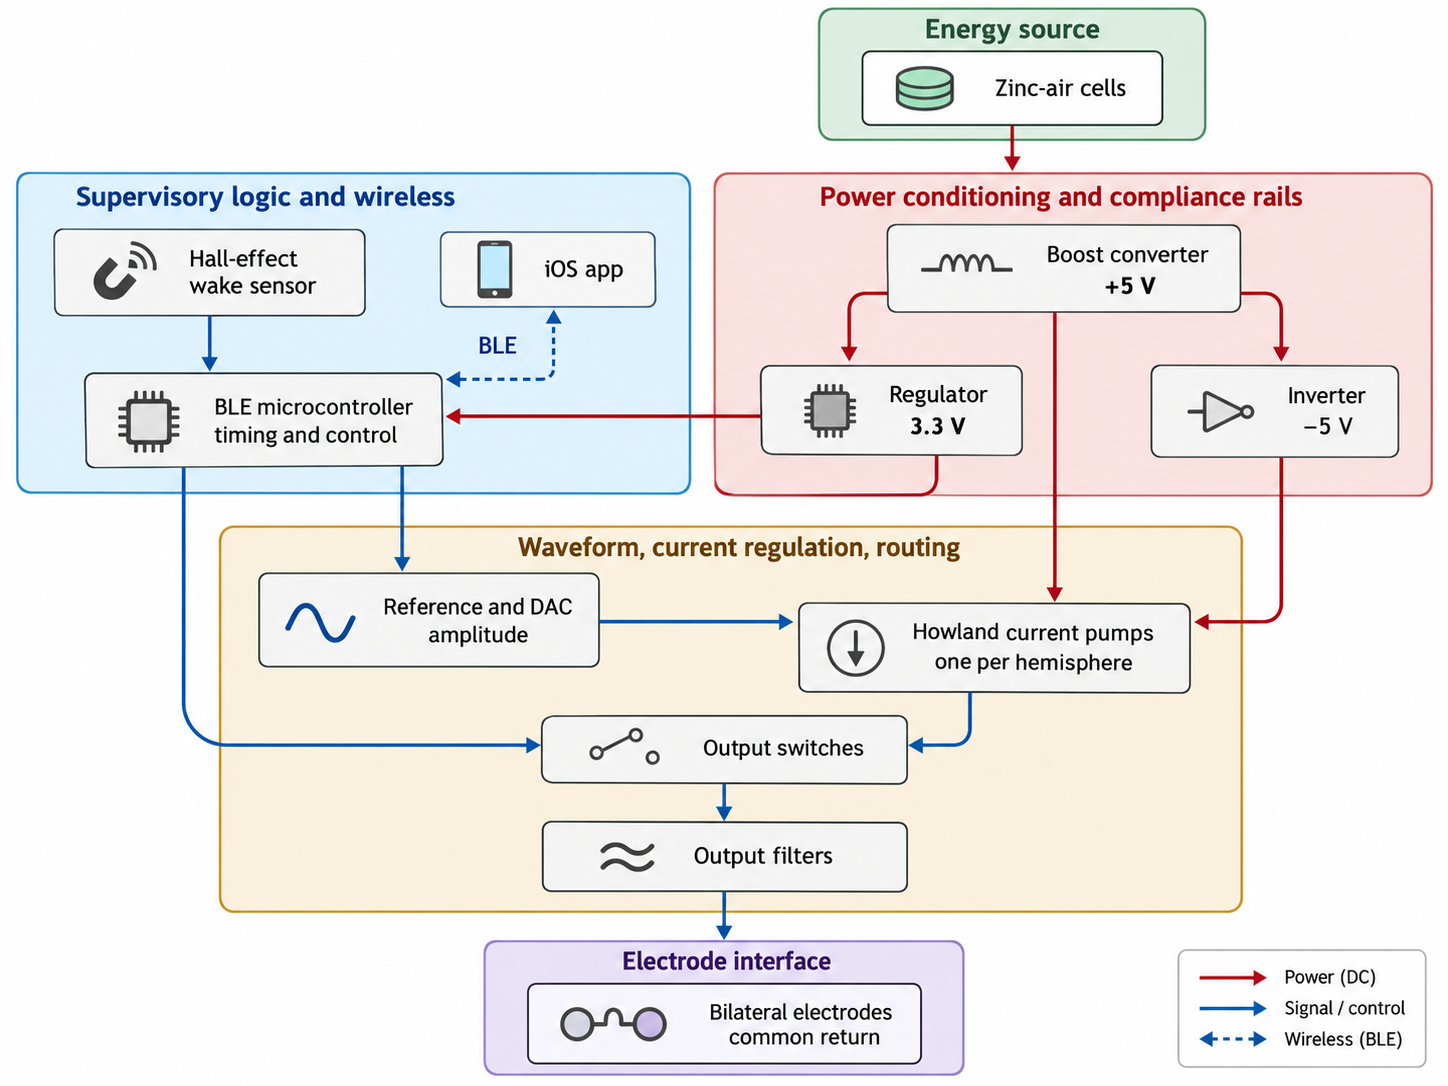
\includegraphics[width=4.5in,height=0.6\textheight,keepaspectratio]{figures/fig1_architecture.png}
\end{center}
\end{minipage}

\noindent\begin{minipage}{\linewidth}
\textbf{Figure 2. FLEX-DBS hardware.} \emph{(A)} Assembled device viewed from above; scale bar, 10 mm. P, break-away programming tab carrying the Tag-Connect TC2050 footprint, which can be cut off after firmware is loaded. \emph{(B)} Rendering of the device from below with the snap-on shroud, showing the two zinc-air cell holders and the electrode connector. The board measures 19.5 mm × 22.5 mm excluding the programming tab, and the assembled device is 8.72 mm thick.

\begin{center}
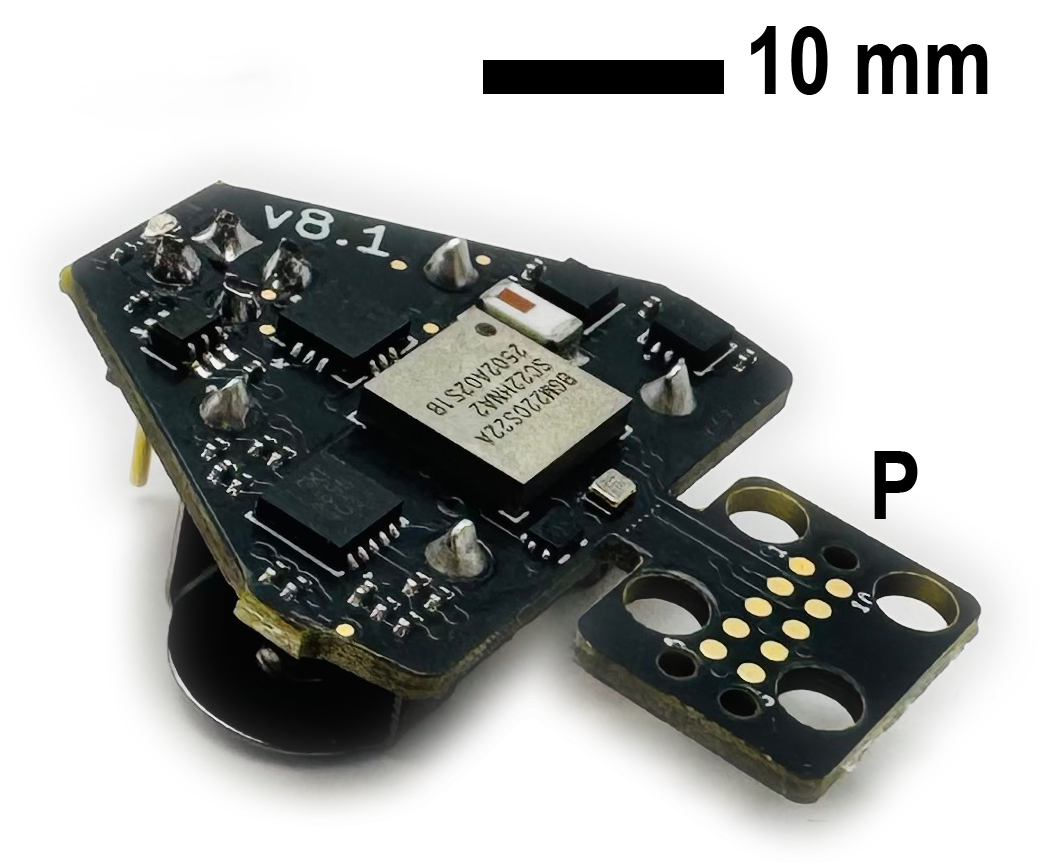
\includegraphics[width=2.9in,height=2.6in,keepaspectratio]{figures/FLEX-DBS_deviceScale.jpg}
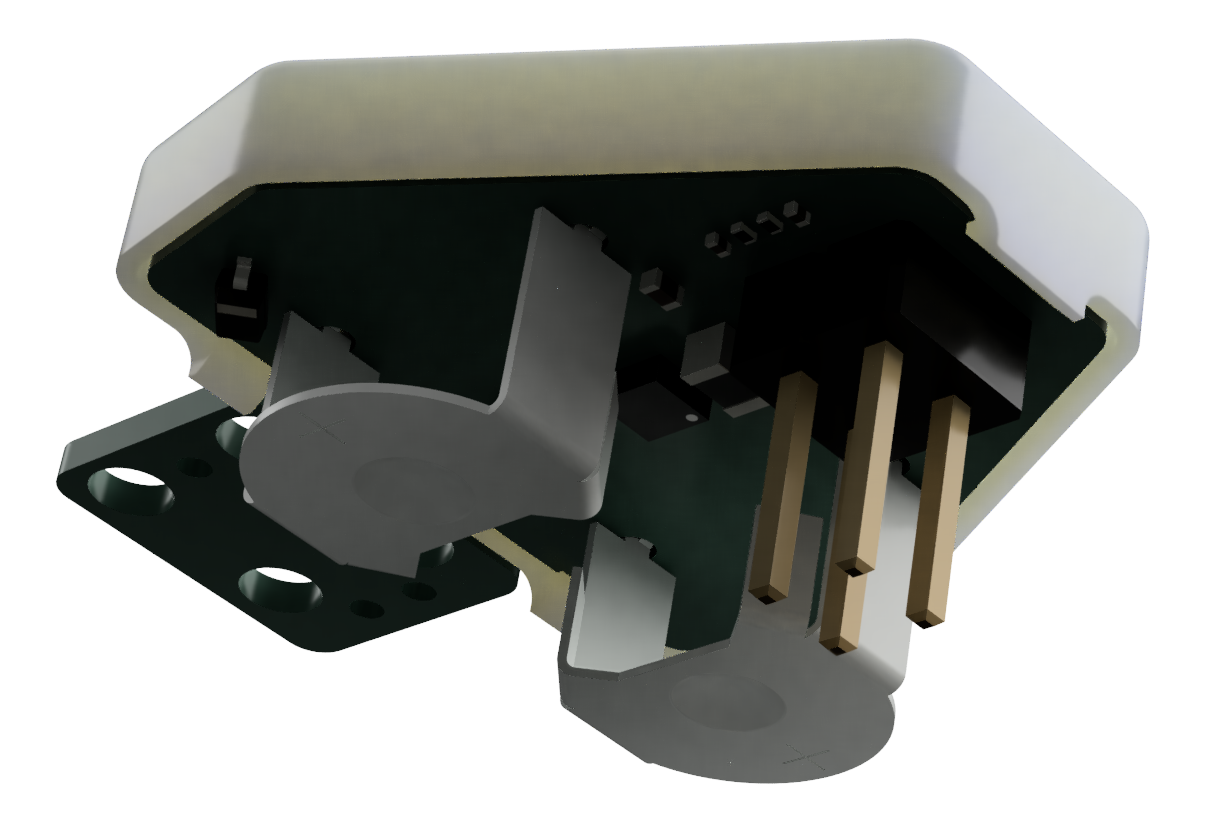
\includegraphics[width=2.9in,height=2.6in,keepaspectratio]{figures/FLEX-DBS_3D_render.png}
\end{center}
\end{minipage}

\noindent\begin{minipage}{\linewidth}
\textbf{Figure 3. MouseCap iOS application.} \emph{(Left)} Continuous mode: amplitude (percent of full scale and nominal current into 1 kΩ), pulse duration and frequency sliders; device ID, firmware version and battery indicator; activation toggle, Sync, LED and Read controls. \emph{(Right)} Burst mode: burst period, intra-burst frequency and burst duration with unit selection. Representative settings are shown (50 \%, 90 µs, 130 Hz; 30 s burst period, 10 s burst duration). Displayed values are settings; delivered values are given in Table 2.

\begin{center}
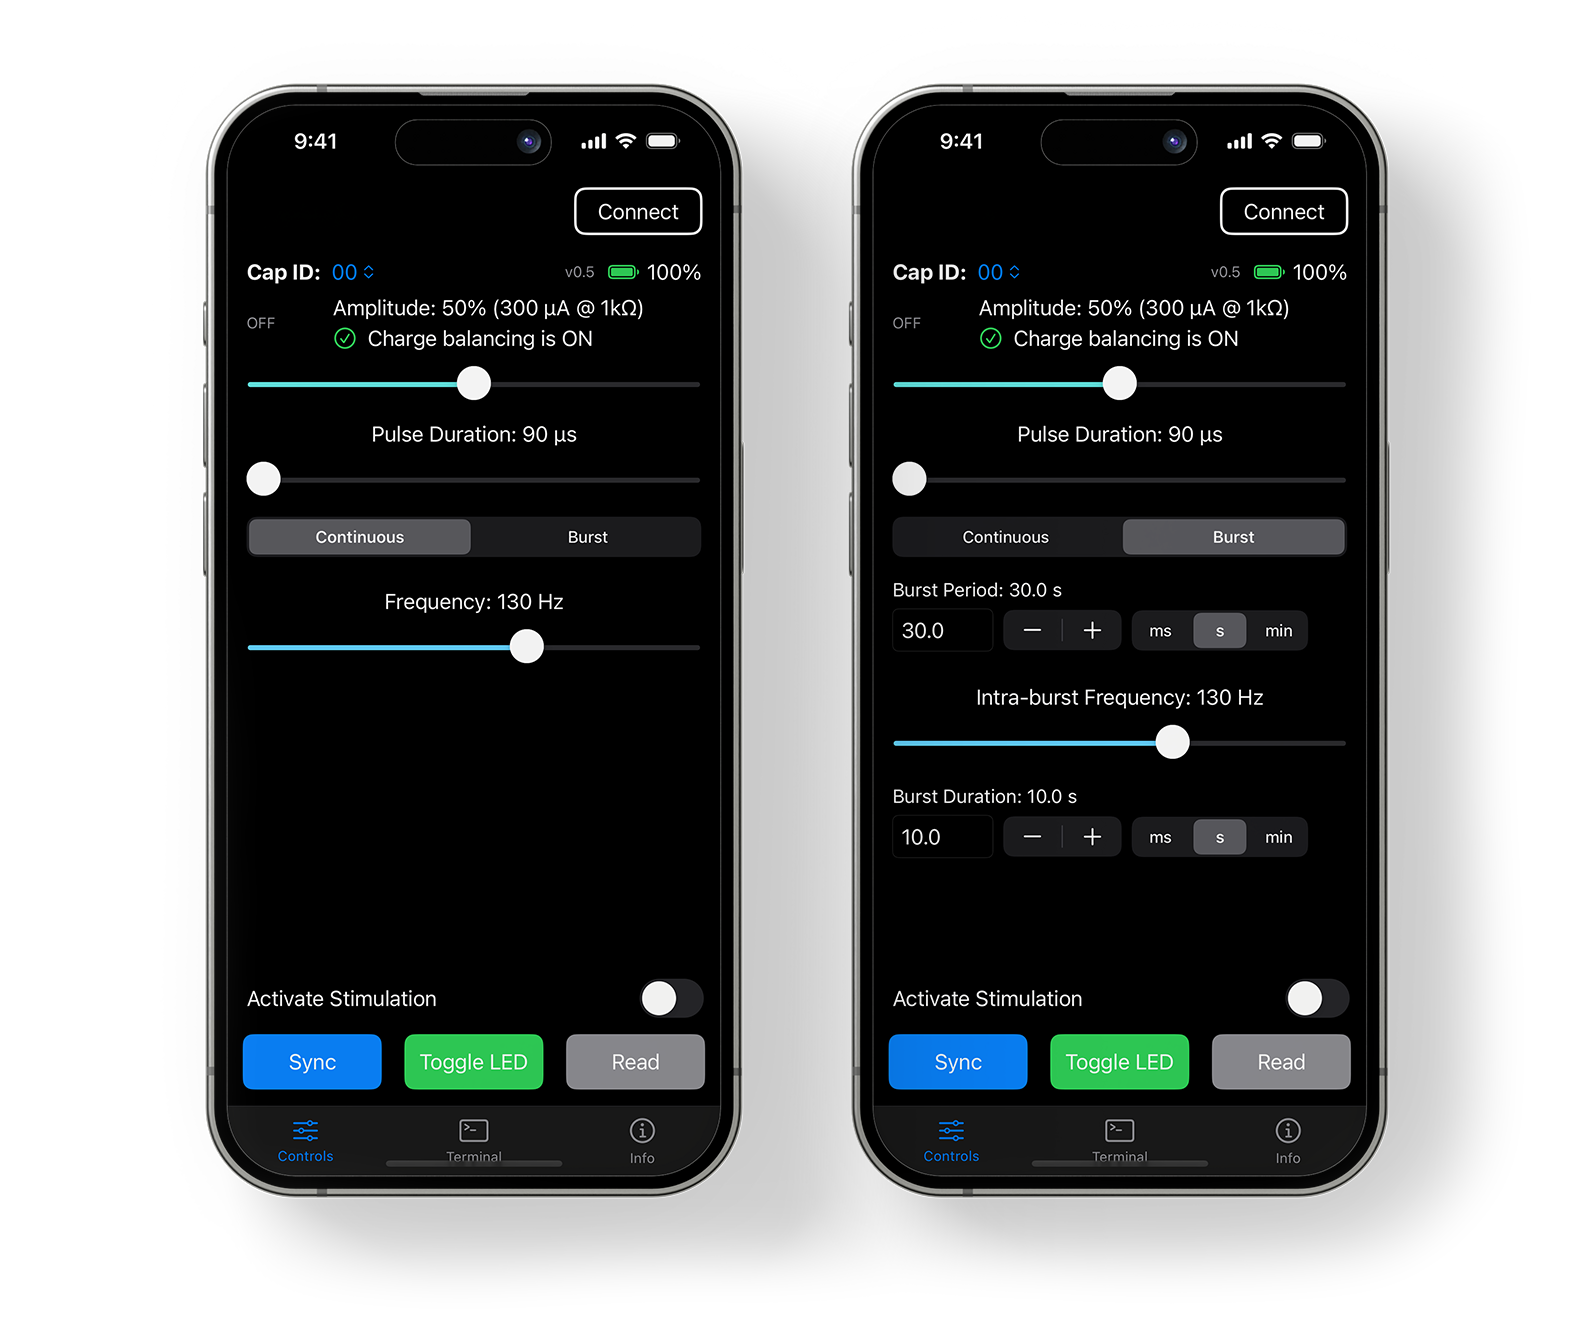
\includegraphics[width=5.5in]{figures/FLEX-DBS_iPhoneRenders.png}
\end{center}
\end{minipage}

\noindent\begin{minipage}{\linewidth}
\textbf{Figure 4. In-vivo electrode impedance and the compliance envelope.} \emph{(A)} Impedance of implanted platinum electrodes from 1 to 8 weeks after implantation, a pulse-derived estimate of the effective load computed as pulse voltage over delivered current with 10 µA, 450 µs pulses (five readings averaged per electrode and session). Points show the mean ± SD across five electrodes from three mice; three of eight implanted electrodes were excluded (Section 3.2). \emph{(B)} Top: largest regulated current of FLEX-DBS as a function of load impedance, $I_\mathrm{max} = 4.6\ \mathrm{V} / (|Z| + 2.66\ \mathrm{k}\Omega)$, with the swing measured into 47 kΩ. The gray band spans the range of weekly mean impedances in (A), 43--54 kΩ, and the dashed lines project it to the corresponding current range, 81--101 µA; the dotted line marks the 100 µA reference protocol. Bottom: weekly mean ± SD impedance on the same impedance axis, colored from week 1 (bottom) to week 8 (top).

\begin{center}
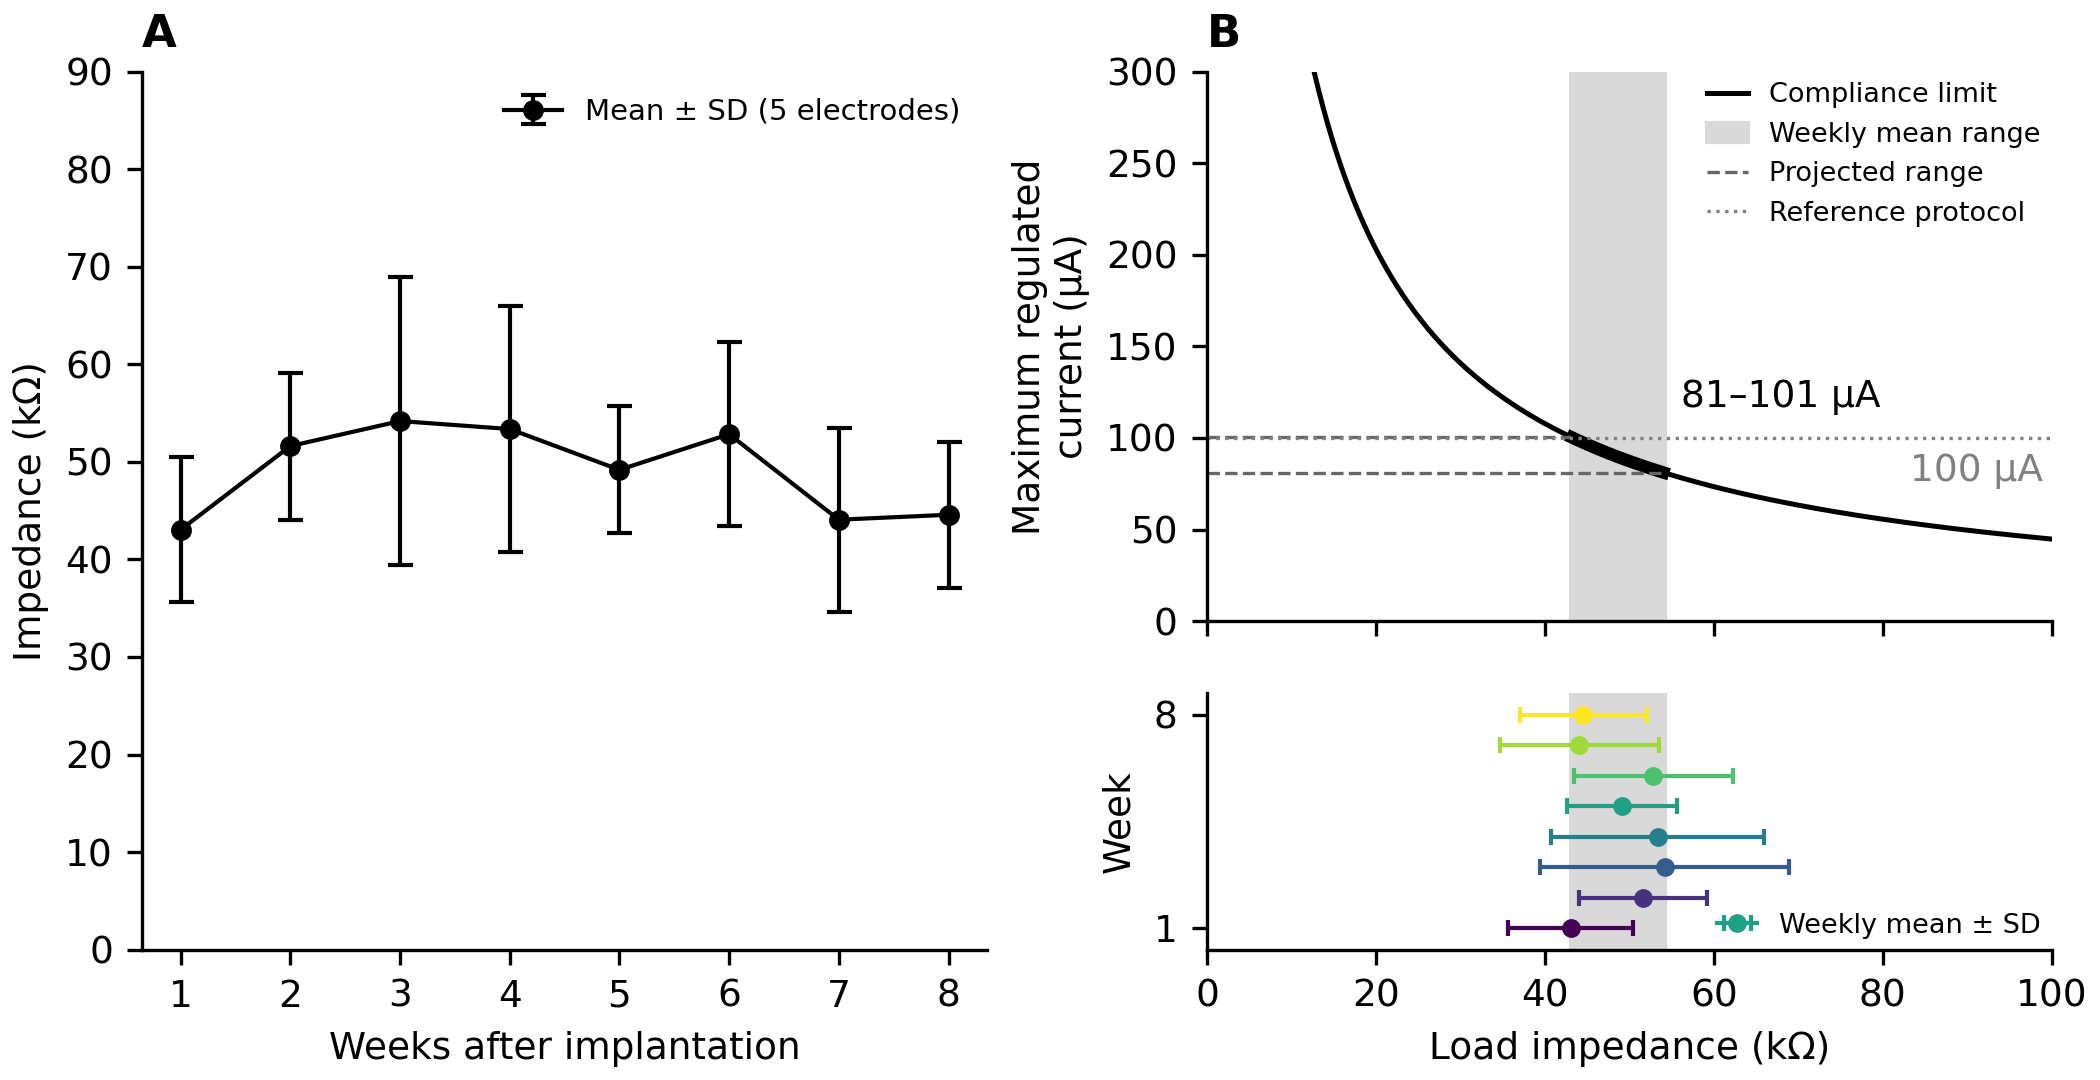
\includegraphics[width=\linewidth]{figures/fig4_impedance.png}
\end{center}
\end{minipage}

\noindent\begin{minipage}{\linewidth}
\textbf{Figure 5. Bench output into 1 kΩ and 47 kΩ loads.} Both outputs of a FLEX-DBS device (firmware v0.5) were loaded with 1 kΩ, or with a nominal 47 kΩ within the in-vivo load range, and one output was recorded at 500 kHz for $\sim$11 s at each of three amplitude settings (10, 50 and 100 \%; 180 µs, 130 Hz). Current is the voltage across the load divided by the load resistance, after a 38 µs median filter that removes range-switching artifacts of the meter. \emph{(A)} Median pulse at each setting into 1 kΩ (1545--1602 pulses); the 5th--95th percentile band lies within the line width. Shading marks the set stimulating (180 µs) and recovery (900 µs) phases. \emph{(B)} Mean plateau current of the stimulating phase against the amplitude setting into 1 kΩ (filled) and 47 kΩ (open). The dotted line marks the 92.6 µA compliance limit into 47 kΩ; the 10 \% point at 47 kΩ is reduced by slow edges. \emph{(C)} Charge in each phase of the median pulse at 1 kΩ (solid) and 47 kΩ (hatched), and the mean net charge over a full period (labeled; nC, nanocoulombs). At every setting and load the delivered frequency was 142.5 Hz; into 1 kΩ the stimulating phase lasted 238--254 µs and the recovery phase 854--878 µs.

\begin{center}
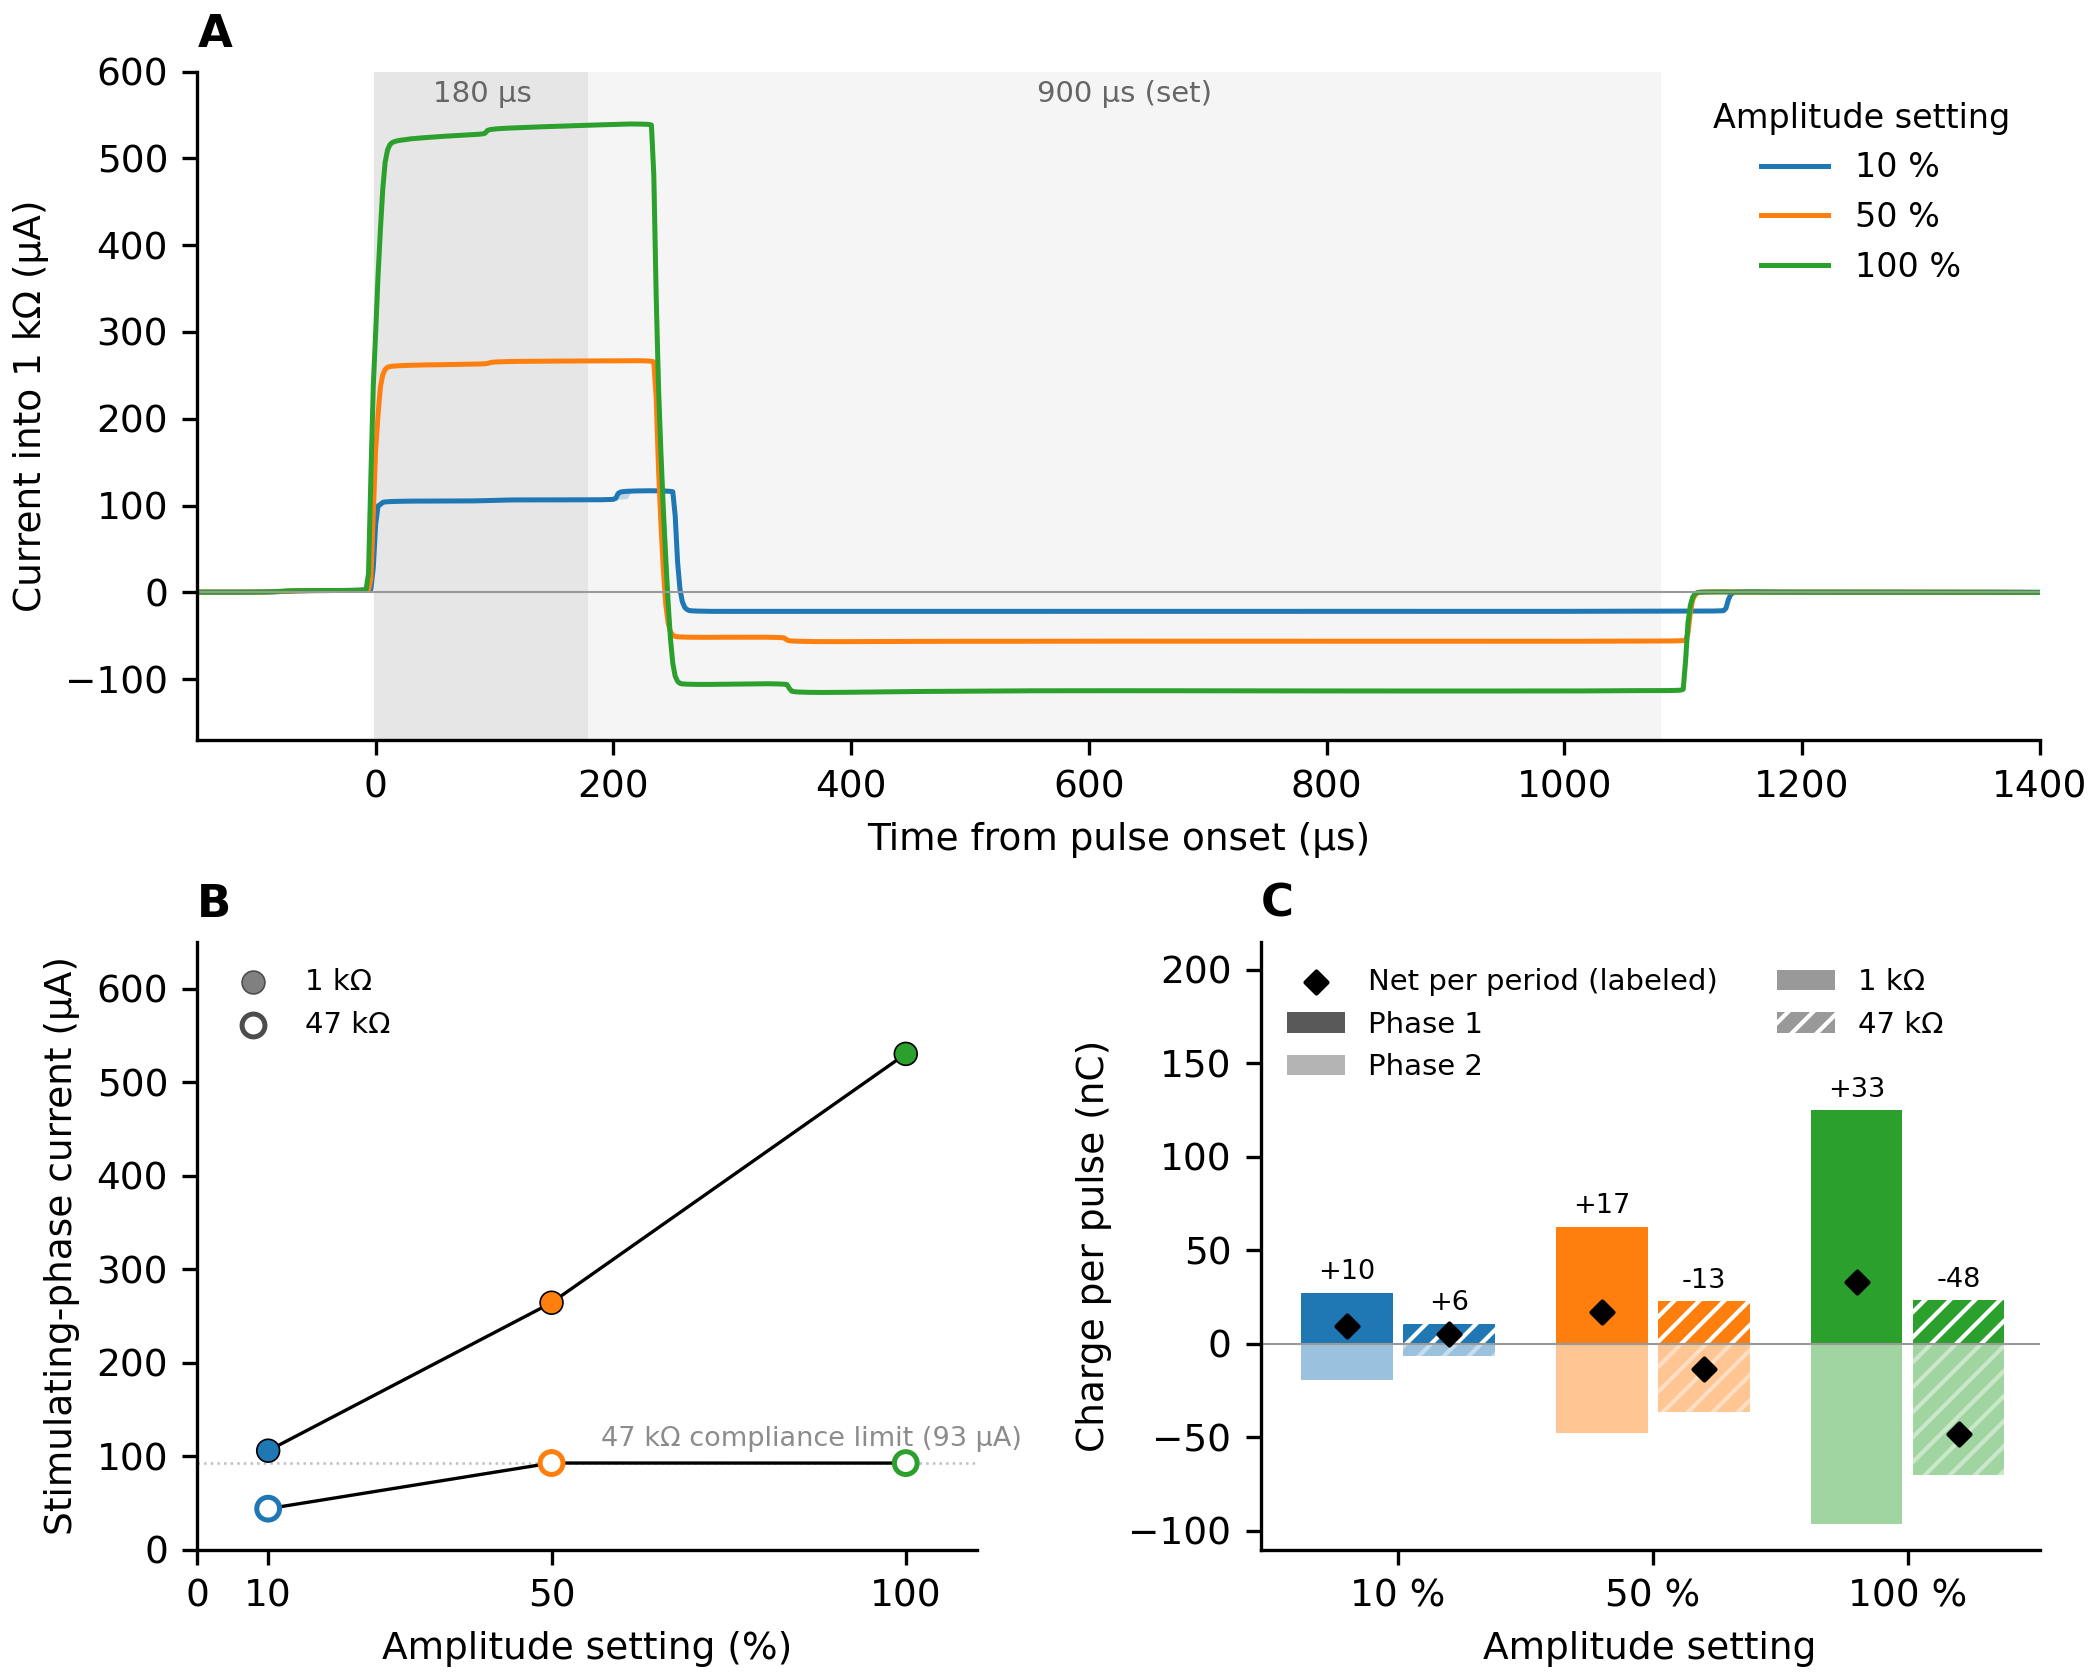
\includegraphics[width=\linewidth]{figures/fig5_bench.png}
\end{center}
\end{minipage}
